%-----------------------------------------------------------------------------------------------------------------------------------------------%
%	The MIT License (MIT)
%
%	Copyright (c) 2019 Jan Küster
%
%	Permission is hereby granted, free of charge, to any person obtaining a copy
%	of this software and associated documentation files (the "Software"), to deal
%	in the Software without restriction, including without limitation the rights
%	to use, copy, modify, merge, publish, distribute, sublicense, and/or sell
%	copies of the Software, and to permit persons to whom the Software is
%	furnished to do so, subject to the following conditions:
%	
%	THE SOFTWARE IS PROVIDED "AS IS", WITHOUT WARRANTY OF ANY KIND, EXPRESS OR
%	IMPLIED, INCLUDING BUT NOT LIMITED TO THE WARRANTIES OF MERCHANTABILITY,
%	FITNESS FOR A PARTICULAR PURPOSE AND NONINFRINGEMENT. IN NO EVENT SHALL THE
%	AUTHORS OR COPYRIGHT HOLDERS BE LIABLE FOR ANY CLAIM, DAMAGES OR OTHER
%	LIABILITY, WHETHER IN AN ACTION OF CONTRACT, TORT OR OTHERWISE, ARISING FROM,
%	OUT OF OR IN CONNECTION WITH THE SOFTWARE OR THE USE OR OTHER DEALINGS IN
%	THE SOFTWARE.
%	
%
%-----------------------------------------------------------------------------------------------------------------------------------------------%


%============================================================================%
%
%	DOCUMENT DEFINITION
%
%============================================================================%

%we use article class because we want to fully customize the page and don't use a cv template
\documentclass[10pt,A4]{article}	


%----------------------------------------------------------------------------------------
%	ENCODING
%----------------------------------------------------------------------------------------

% we use utf8 since we want to build from any machine
\usepackage[utf8]{inputenc}		

%----------------------------------------------------------------------------------------
%	LOGIC
%----------------------------------------------------------------------------------------

% provides \isempty test
\usepackage{xstring, xifthen}

%----------------------------------------------------------------------------------------
%	FONT BASICS
%----------------------------------------------------------------------------------------

% some tex-live fonts - choose your own

%\usepackage[defaultsans]{droidsans}
%\usepackage[default]{comfortaa}
%\usepackage{cmbright}
\usepackage[default]{raleway}
%\usepackage{fetamont}
%\usepackage[default]{gillius}
%\usepackage[light,math]{iwona}
%\usepackage[thin]{roboto} 

% set font default
\renewcommand*\familydefault{\sfdefault} 	
\usepackage[T1]{fontenc}

% more font size definitions
\usepackage{moresize}

%----------------------------------------------------------------------------------------
%	FONT AWESOME ICONS
%---------------------------------------------------------------------------------------- 

% include the fontawesome icon set
\usepackage{fontawesome}

% use to vertically center content
% credits to: http://tex.stackexchange.com/questions/7219/how-to-vertically-center-two-images-next-to-each-other
\newcommand{\vcenteredinclude}[1]{\begingroup
\setbox0=\hbox{\includegraphics{#1}}%
\parbox{\wd0}{\box0}\endgroup}

% use to vertically center content
% credits to: http://tex.stackexchange.com/questions/7219/how-to-vertically-center-two-images-next-to-each-other
\newcommand*{\vcenteredhbox}[1]{\begingroup
\setbox0=\hbox{#1}\parbox{\wd0}{\box0}\endgroup}

% icon shortcut
\newcommand{\icon}[3] { 							
	\makebox(#2, #2){\textcolor{maincol}{\csname fa#1\endcsname}}
}	

% icon with text shortcut
\newcommand{\icontext}[4]{ 						
	\vcenteredhbox{\icon{#1}{#2}{#3}}  \hspace{2pt}  \parbox{0.9\mpwidth}{\textcolor{#4}{#3}}
}

% icon with website url
\newcommand{\iconhref}[5]{ 						
    \vcenteredhbox{\icon{#1}{#2}{#5}}  \hspace{2pt} \href{#4}{\textcolor{#5}{#3}}
}

% icon with email link
\newcommand{\iconemail}[5]{ 						
    \vcenteredhbox{\icon{#1}{#2}{#5}}  \hspace{2pt} \href{mailto:#4}{\textcolor{#5}{#3}}
}

%----------------------------------------------------------------------------------------
%	PAGE LAYOUT  DEFINITIONS
%----------------------------------------------------------------------------------------

% page outer frames (debug-only)
% \usepackage{showframe}		

% we use paracol to display breakable two columns
\usepackage{paracol}

% define page styles using geometry
\usepackage[a4paper]{geometry}

% remove all possible margins
\geometry{top=1cm, bottom=1cm, left=1cm, right=1cm}

\usepackage{fancyhdr}
\pagestyle{empty}

% space between header and content
% \setlength{\headheight}{0pt}

% indentation is zero
\setlength{\parindent}{0mm}

%----------------------------------------------------------------------------------------
%	TABLE /ARRAY DEFINITIONS
%---------------------------------------------------------------------------------------- 

% extended aligning of tabular cells
\usepackage{array}

% custom column right-align with fixed width
% use like p{size} but via x{size}
\newcolumntype{x}[1]{%
>{\raggedleft\hspace{0pt}}p{#1}}%


%----------------------------------------------------------------------------------------
%	GRAPHICS DEFINITIONS
%---------------------------------------------------------------------------------------- 

%for header image
\usepackage{graphicx}

% use this for floating figures
% \usepackage{wrapfig}
% \usepackage{float}
% \floatstyle{boxed} 
% \restylefloat{figure}

%for drawing graphics		
\usepackage{tikz}				
\usetikzlibrary{shapes, backgrounds,mindmap, trees}

%----------------------------------------------------------------------------------------
%	Color DEFINITIONS
%---------------------------------------------------------------------------------------- 
\usepackage{transparent}
\usepackage{color}

% primary color
\definecolor{maincol}{RGB}{ 225, 0, 0 }

% accent color, secondary
% \definecolor{accentcol}{RGB}{ 250, 150, 10 }

% dark color
\definecolor{darkcol}{RGB}{ 70, 70, 70 }

% light color
\definecolor{lightcol}{RGB}{245,245,245}


% Package for links, must be the last package used
\usepackage[hidelinks]{hyperref}

% returns minipage width minus two times \fboxsep
% to keep padding included in width calculations
% can also be used for other boxes / environments
\newcommand{\mpwidth}{\linewidth-\fboxsep-\fboxsep}
	


%============================================================================%
%
%	CV COMMANDS
%
%============================================================================%

%----------------------------------------------------------------------------------------
%	 CV LIST
%----------------------------------------------------------------------------------------

% renders a standard latex list but abstracts away the environment definition (begin/end)
\newcommand{\cvlist}[1] {
	\begin{itemize}{#1}\end{itemize}
}

%----------------------------------------------------------------------------------------
%	 CV TEXT
%----------------------------------------------------------------------------------------

% base class to wrap any text based stuff here. Renders like a paragraph.
% Allows complex commands to be passed, too.
% param 1: *any
\newcommand{\cvtext}[1] {
	\begin{tabular*}{1\mpwidth}{p{0.98\mpwidth}}
		\parbox{1\mpwidth}{#1}
	\end{tabular*}
}

%----------------------------------------------------------------------------------------
%	CV SECTION
%----------------------------------------------------------------------------------------

% Renders a a CV section headline with a nice underline in main color.
% param 1: section title
\newcommand{\cvsection}[1] {
	\vspace{14pt}
	\cvtext{
		\textbf{\LARGE{\textcolor{darkcol}{\uppercase{#1}}}}\\[-4pt]
		\textcolor{maincol}{ \rule{0.1\textwidth}{2pt} } \\
	}
}

%----------------------------------------------------------------------------------------
%	META SKILL
%----------------------------------------------------------------------------------------

% Renders a progress-bar to indicate a certain skill in percent.
% param 1: name of the skill / tech / etc.
% param 2: level (for example in years)
% param 3: percent, values range from 0 to 1
\newcommand{\cvskill}[3] {
	\begin{tabular*}{1\mpwidth}{p{0.72\mpwidth}  r}
 		\textcolor{black}{\textbf{#1}} & \textcolor{maincol}{#2}\\
	\end{tabular*}%
	
	\hspace{4pt}
	\begin{tikzpicture}[scale=1,rounded corners=2pt,very thin]
		\fill [lightcol] (0,0) rectangle (1\mpwidth, 0.15);
		\fill [maincol] (0,0) rectangle (#3\mpwidth, 0.15);
  	\end{tikzpicture}%
}


%----------------------------------------------------------------------------------------
%	 CV EVENT
%----------------------------------------------------------------------------------------

% Renders a table and a paragraph (cvtext) wrapped in a parbox (to ensure minimum content
% is glued together when a pagebreak appears).
% Additional Information can be passed in text or list form (or other environments).
% the work you did
% param 1: time-frame i.e. Sep 14 - Jan 15 etc.
% param 2:	 event name (job position etc.)
% param 3: Customer, Employer, Industry
% param 4: Short description
% param 5: work done (optional)
% param 6: technologies include (optional)
% param 7: achievements (optional)
\newcommand{\cvevent}[7] {
	
	% we wrap this part in a parbox, so title and description are not separated on a pagebreak
	% if you need more control on page breaks, remove the parbox
	\parbox{\mpwidth}{
		\begin{tabular*}{1\mpwidth}{p{0.72\mpwidth}  r}
	 		\textcolor{black}{\textbf{#2}} & \colorbox{maincol}{\makebox[0.25\mpwidth]{\textcolor{white}{#1}}} \\
			\textcolor{maincol}{\textbf{#3}} & \\
		\end{tabular*}\\[8pt]
	
		\ifthenelse{\isempty{#4}}{}{
			\cvtext{#4}\\
		}
	}

	\ifthenelse{\isempty{#5}}{}{
		\vspace{9pt}
		{#5}
	}

	\ifthenelse{\isempty{#6}}{}{
		\vspace{9pt}
		\cvtext{\textbf{Technologies include:}}\\
		{#6}
	}

	\ifthenelse{\isempty{#7}}{}{
		\vspace{9pt}
		\cvtext{\textbf{Achievements include:}}\\
		{#7}
	}
	\vspace{14pt}
}

%----------------------------------------------------------------------------------------
%	 CV META EVENT
%----------------------------------------------------------------------------------------

% Renders a CV event on the sidebar
% param 1: title
% param 2: subtitle (optional)
% param 3: customer, employer, etc,. (optional)
% param 4: info text (optional)
\newcommand{\cvmetaevent}[4] {
	\textcolor{maincol} {\cvtext{\textbf{\begin{flushleft}#1\end{flushleft}}}}

	\ifthenelse{\isempty{#2}}{}{
	\textcolor{darkcol} {\cvtext{\textbf{#2}} }
	}

	\ifthenelse{\isempty{#3}}{}{
		\cvtext{{ \textcolor{darkcol} {#3} }}\\
	}

	\cvtext{#4}\\[14pt]
}

%---------------------------------------------------------------------------------------
%	QR CODE
%----------------------------------------------------------------------------------------

% Renders a qrcode image (centered, relative to the parentwidth)
% param 1: percent width, from 0 to 1
\newcommand{\cvqrcode}[1] {
	\begin{center}
	\href{https://www.kristoferpearson.com}{
		
\includegraphics[width={#1}\mpwidth]{qrcode}
		}
	\end{center}
}


%============================================================================%
%
%
%
%	DOCUMENT CONTENT
%
%
%
%============================================================================%
\begin{document}
\columnratio{0.31}
\setlength{\columnsep}{2.2em}
\setlength{\columnseprule}{4pt}
\colseprulecolor{lightcol}
\begin{paracol}{2}
\begin{leftcolumn}
%---------------------------------------------------------------------------------------
%	META IMAGE
%----------------------------------------------------------------------------------------
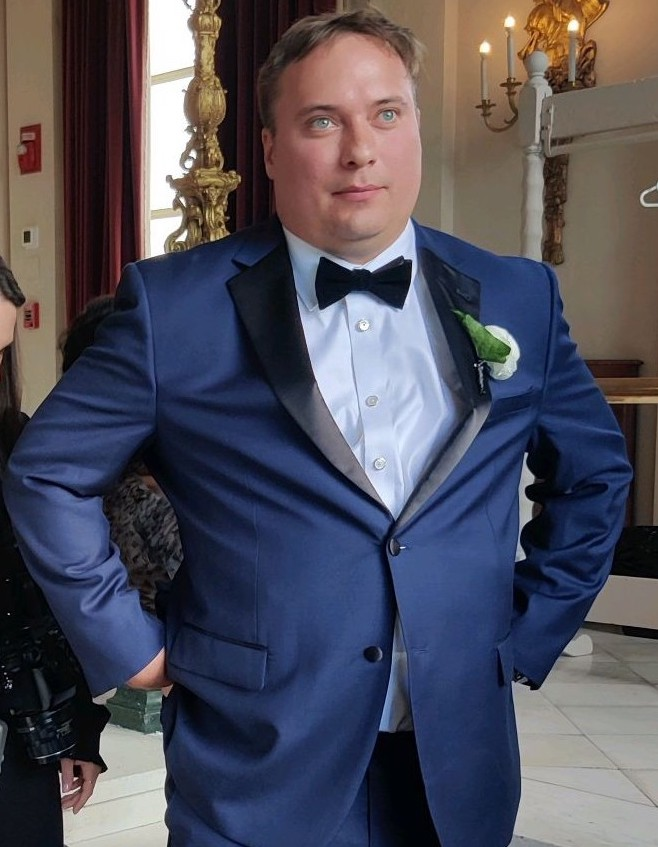
\includegraphics[width=\linewidth]{me.jpg}	%trimming relative to image size

%---------------------------------------------------------------------------------------
%	META SKILLS
%----------------------------------------------------------------------------------------
\cvsection{SKILLS}

\cvskill{SQL Server} {8+ yrs} {1} \\[-2pt]

\cvskill{Java} {3+ yrs} {1} \\[-2pt]

\cvskill{Javascript} {3+ yrs} {0.69} \\[-2pt]

\cvskill{Python} {4+ yrs} {0.8} \\[-2pt]

\cvskill{Html/CSS} {3+ yrs} {0.72} \\[-2pt]

\cvskill{React} {3+ yrs} {0.69} \\[-2pt]

\cvskill{GIT} {3+ yrs} {1} \\[-2pt]



\vfill\null
\cvsection{CONTACT}
	
\icontext{MapMarker}{12}{70 Endicott St. \#601\\Norwood, MA 02062}{black}\\[6pt]
\icontext{MobilePhone}{12}{508-208-0210}{black}\\[6pt]
\iconemail{Envelope}{12}{pearsonk27@gmail.com}{pearsonk27@gmail.com}{black}\\[6pt]

\vfill\null
\cvqrcode{0.7}

%---------------------------------------------------------------------------------------
%	EDUCATION
%----------------------------------------------------------------------------------------
\newpage
\cvsection{EDUCATION}

\cvmetaevent
{2010 - 2014}
{Boston College}
{Bachelor of Arts - Economics, Minor in Mathematics}
{Main curriculum priority was in quantitative/analytical courses such as Econometrics, Statistics, Probability, Integrated Math and Physics, and Sports Econometrics. \\

Many courses required aptitude in programming languages and software such as STATA, Excel, R, Python, LaTeX and more. \\

Chosen to be a Research Assistant where in empirical research on media and digital imagery markets, including research on industry background and data processing and analysis. \\

Also participated in the Investment Club, Lacrosse Club, and studied abroad.}

\cvsection{AWARDS}

\cvmetaevent
{2018}
{Employee of the Year Award}
{}
{Awarded for my integral role in improving the product offerings to fit the largest client's needs.}

\cvmetaevent
{2018}
{Patrick J Martin Committe Chair}
{}
{Identified employees throughout the organization who displayed talent and passion in their given roles, working with 5 committee members to select award recipient.}

\vfill\null
\cvqrcode{0.7}

%---------------------------------------------------------------------------------------
%	CERTIFICATION
%----------------------------------------------------------------------------------------
\newpage
\cvsection{CERTIFICATIONS}

\cvmetaevent
{OCA - Java SE 8 Programmer}
{}
{}
{Issued October 2020}

\cvsection{COURSES}

\cvmetaevent
{2020}
{Java for Data Scientists Essential Training}
{}
{}

\cvmetaevent
{2020}
{Learning JDBC}
{}
{}

\cvmetaevent
{}
{}
{To find the most up-to-date list of my courses I've taken, visit my LinkedIn linked to from my portfolio at kristoferpearson.com or follow my QR Code on this resume.}
{}

\vfill\null
\cvqrcode{0.7}

\newpage
\cvsection{PERSONAL PROJECTS}

\cvmetaevent
{WebExecuter}
{}
{}
{Project I use to automatically pay my town utility/cable bills. UI starts jobs on my Raspberry Pi that hosts the database, frontend, and scripts}

\cvmetaevent
{cheatsheet.io}
{}
{}
{CRUD app utilizing Java Spring Boot, React, and Postgresql. The frontend and backend are each standalone projects.}

\cvmetaevent
{wordlecheat}
{}
{}
{My attempt at finding the optimal strategy at Wordle. The application "plays the game" over and over again with different strategies, recording what happens and analyzes the data}

\cvmetaevent
{}
{}
{These projects can be found on my Github page. You can get there by going to my portfolio at kristoferpearson.com or following my QR Code on this resume.}
{}

\vfill

\mbox{} % hotfix to place qrcode on the bottom when there are not other elements
\vfill
\cvqrcode{0.7}

\end{leftcolumn}
\begin{rightcolumn}
%---------------------------------------------------------------------------------------
%	TITLE  HEADER
%----------------------------------------------------------------------------------------
\fcolorbox{white}{darkcol}{\begin{minipage}[c][3.5cm][c]{1\mpwidth}
	\begin {center}
		\HUGE{ \textbf{ \textcolor{white}{ \uppercase{ KRIS PEARSON } } } } \\[-24pt]
		\textcolor{white}{ \rule{0.1\textwidth}{1.25pt} } \\[4pt]
		\large{ \textcolor{white} {Software Engineer} }
	\end {center}
\end{minipage}} \\[14pt]
\vspace{-12pt}

%---------------------------------------------------------------------------------------
%	PROFILE
%----------------------------------------------------------------------------------------
\vfill\null
\cvsection{PROFILE}

\cvtext{Software Engineer with a strong technical and analytical skills and professional demeanor.\\

Strong interest in big data, automated QA, and application development.\\

Has worked in many different companies with many different methodologies and personalities. Adapting while keeping the same likable personality and positive attitude is an undeniable strength.\\

}

%---------------------------------------------------------------------------------------
%	WORK EXPERIENCE
%----------------------------------------------------------------------------------------
\vfill\null
\cvsection{WORK EXPERIENCE}

\cvevent
	{Apr 2022 - NOW}
	{SBE Vision}
	{Software Engineer}
	{A large micro-service architecture built with Java Spring Boot applications orchestrated by Kubernetes.}
	{\cvlist{
		\item Creation of a full-trip tests of the stack managed by a REST API application to host requests called in a larger Postman Collection hit regularly by a Newman Runner.
		\item Maintain the Microsoft Excel Adapter/Plugin
		\item Build out reporting for Elasticsearch
	}}
	{\cvlist {
		\item Java Spring Boot for all backend services
		\item SQL Server and MongoDB for data persistence
		\item Angular for the easy frontend interaction
		\item Kubernetes + Docker for deployments
		\item gRPC, REST API, and Rabbit for service communication
		\item Git for versioning
		\item Git Lab for CI/CD
	}}
	{}

\vfill\null
\cvevent
	{2019 - 2022}
	{Vestmark}
	{Full Stack Software Engineer}
	{Application development on a Java Spring Boot monolithic proprietary investment platform.}
	{\cvlist{
		\item Correct bugs in Vestmarkone during release level testing
		\item Build Selenium tests in the separate Python project
		\item Fixes to client specific data integrations utilizing a proprietary data manipulation API
	}}
	{\cvlist {
		\item Java, SQL Server, and React/Javascript for application development
		\item Terragrunt, AWS and Docker for application deployment
		\item Python using the Selenium library for automated web testing
		\item Apache Camel and Karaf for Data Integration micro-services development
		\item Git for versioning
		\item Jenkins for CI/CD
	}}
	{\cvlist{
		\item Development of new data integration framework using Apache Camel and Karaf
		\item Promoted from Associate SWE to SWE in January 2021
		\item Various user stories implementing Product Level Security Substitutes
	}}

\vfill\null
\cvevent
	{2017 - 2019}
	{Connance / Waystar}
	{Senior Data Integration Engineer}
	{Develop solutions to solve hospital client revenue cycle needs.}
	{\cvlist{
		\item Code and test client specific work aiming to manage sensitive hospital patient account data
		\item Build tools and automation meant to increase the effectiveness and efficiency of the team
		\item Build and design new frameworks for managing common client needs, train engineers on how to use and improve the framework
	}}
	{\cvlist {
		\item Transact SQL for report building, database updates, and functional logic in business rules
		\item SSIS and Powershell for data integration jobs
		\item C\# and Perl for data manipulation during data ingress and egress
		\item Windows Task Scheduler and SQL Server Agent for job scheduling
		\item TFS for versioning
	}}
	{\cvlist{
		\item Assisted in building and improving ActionRules - a replacement for Connance's business rules engine. ActionRules is a configurable batch SQL script moving accounts to various debt collection stages according to various actions taken, inclusion criteria, and exclusion criteria specified by the client in the UI.
		\item Built out UI utilizing MVC framework
		\item Built and helped test performance improvements needed to handle the load given by Waystar's largest client, who is 10 times larger than any other client serviced.
		\item Made Production Engineer Team Lead (3/2019)
		\item Won Employee of the Year award (12/2018)
		\item Patrick J Martin Award Committee Chair (9/2018)
	}}

\vfill\null
\cvevent
	{2014 - 2017}
	{Analyst / Product Manager}
	{Definitive Healthcare}
	{Key technical contributor on many projects building out the company's product offerings and increasing efficiency and effectiveness in various company operations.}
	{\cvlist{
		\item Managed, assisted, and trained (7) analysts in the methodology used to build the proprietary user-friendly web-based application, which consolidates various types of healthcare provider focused data to aid healthcare focused industries.
		\item Managed and assisted the development and maintenance of software.
		\item Delegated or solved all product errors. Quickly identified the source of any errors, determined the level of skill needed to solve the problem, and assigned accordingly.
		\item Team lead for all new technology, product rollouts (one product rollout per month), coding methodology, and database administration.
	}}
	{\cvlist {
		\item SQL Server for ETL, report generation and business logic
		\item Windows Command line
		\item SSIS, C\#, Visual Basic for ETL and report generation
		\item Visual Studio for UI development
		\item Powershell for reporting job execution
		\item ASP.NET, HTML, CSS for UI development and data entry form development
		\item Microsoft Access for data entry form development
	}}
	{\cvlist{
		\item Developed SSIS package and method to build automatically refreshing reports for clients, significantly improving efficiency of company FTP site development process (estimated 75\% less time needed to complete/maintain FTP sites). Process utilized SQL Server view generation and a C\# script.
		\item Developed re-useable PowerShell script that loads data to a client's SFTP server that retries after connection failures, logs output to a .txt file, emails client to confirm data load completion, can be set to run every month, drastically cutting down on employee work necessary
		\item Developed a Master Data matching process using a fuzzy lookup, used to link client data to company data. Regression analysis built into the script to weigh methods used by success rate.
		\item Optimized the company's Population Health queries by adding primary keys and indexes to the tables, as well as redesigning the queries so that there is a high amount of parallelism. Prior to changes, 1 query took 2 minutes, 4 of the same queries at once took 8 minutes, after the changes, 1 query took 4 seconds, 4 of the same queries at once took 8 seconds.
	}}

% hotfixes to create fake-space to ensure the whole height is used
\mbox{}
\vfill
\mbox{}
\vfill
\mbox{}
\vfill
\mbox{}
\end{rightcolumn}
\end{paracol}
\end{document}

